\subsection{7.6 Arrhenius Equation}
    \vspace*{0.5em}
    $\alpha A + \beta B + \gamma C \longrightarrow \text{products}$\\
    $\text{Rate} = k[A]^m [B]^n [C]^p$

    \mathbox{
        k(T) = \underbrace{(\parbox{0.8cm}{\centering\tiny collisions\\per time})*(\parbox{1.65cm}{\centering\tiny fraction of collisions\\properly oriented})}_{\vphantom{* exp[\frac{-E_a}{R T}]} \parbox{0.8cm}{\centering $A$}}
        * \underbrace{(\parbox{1.7cm}{\centering\tiny fraction of molecules\\with $E>E_a$})}_{\parbox{1.7cm}{\raggedright $*\; exp[\frac{-E_a}{R T}]$}}
    }

    $A$ is a "frequency factor", assumed $T$-independent
    \vspace*{0.5em}

    \begin{minipage}{0.99\linewidth}
        \begin{minipage}{0.49\linewidth}
            \centerline{$ln(k) = \frac{-E_a}{R} \frac{1}{T} + ln(A)$}
        \end{minipage}
        \begin{minipage}{0.49\linewidth}
            \centerline{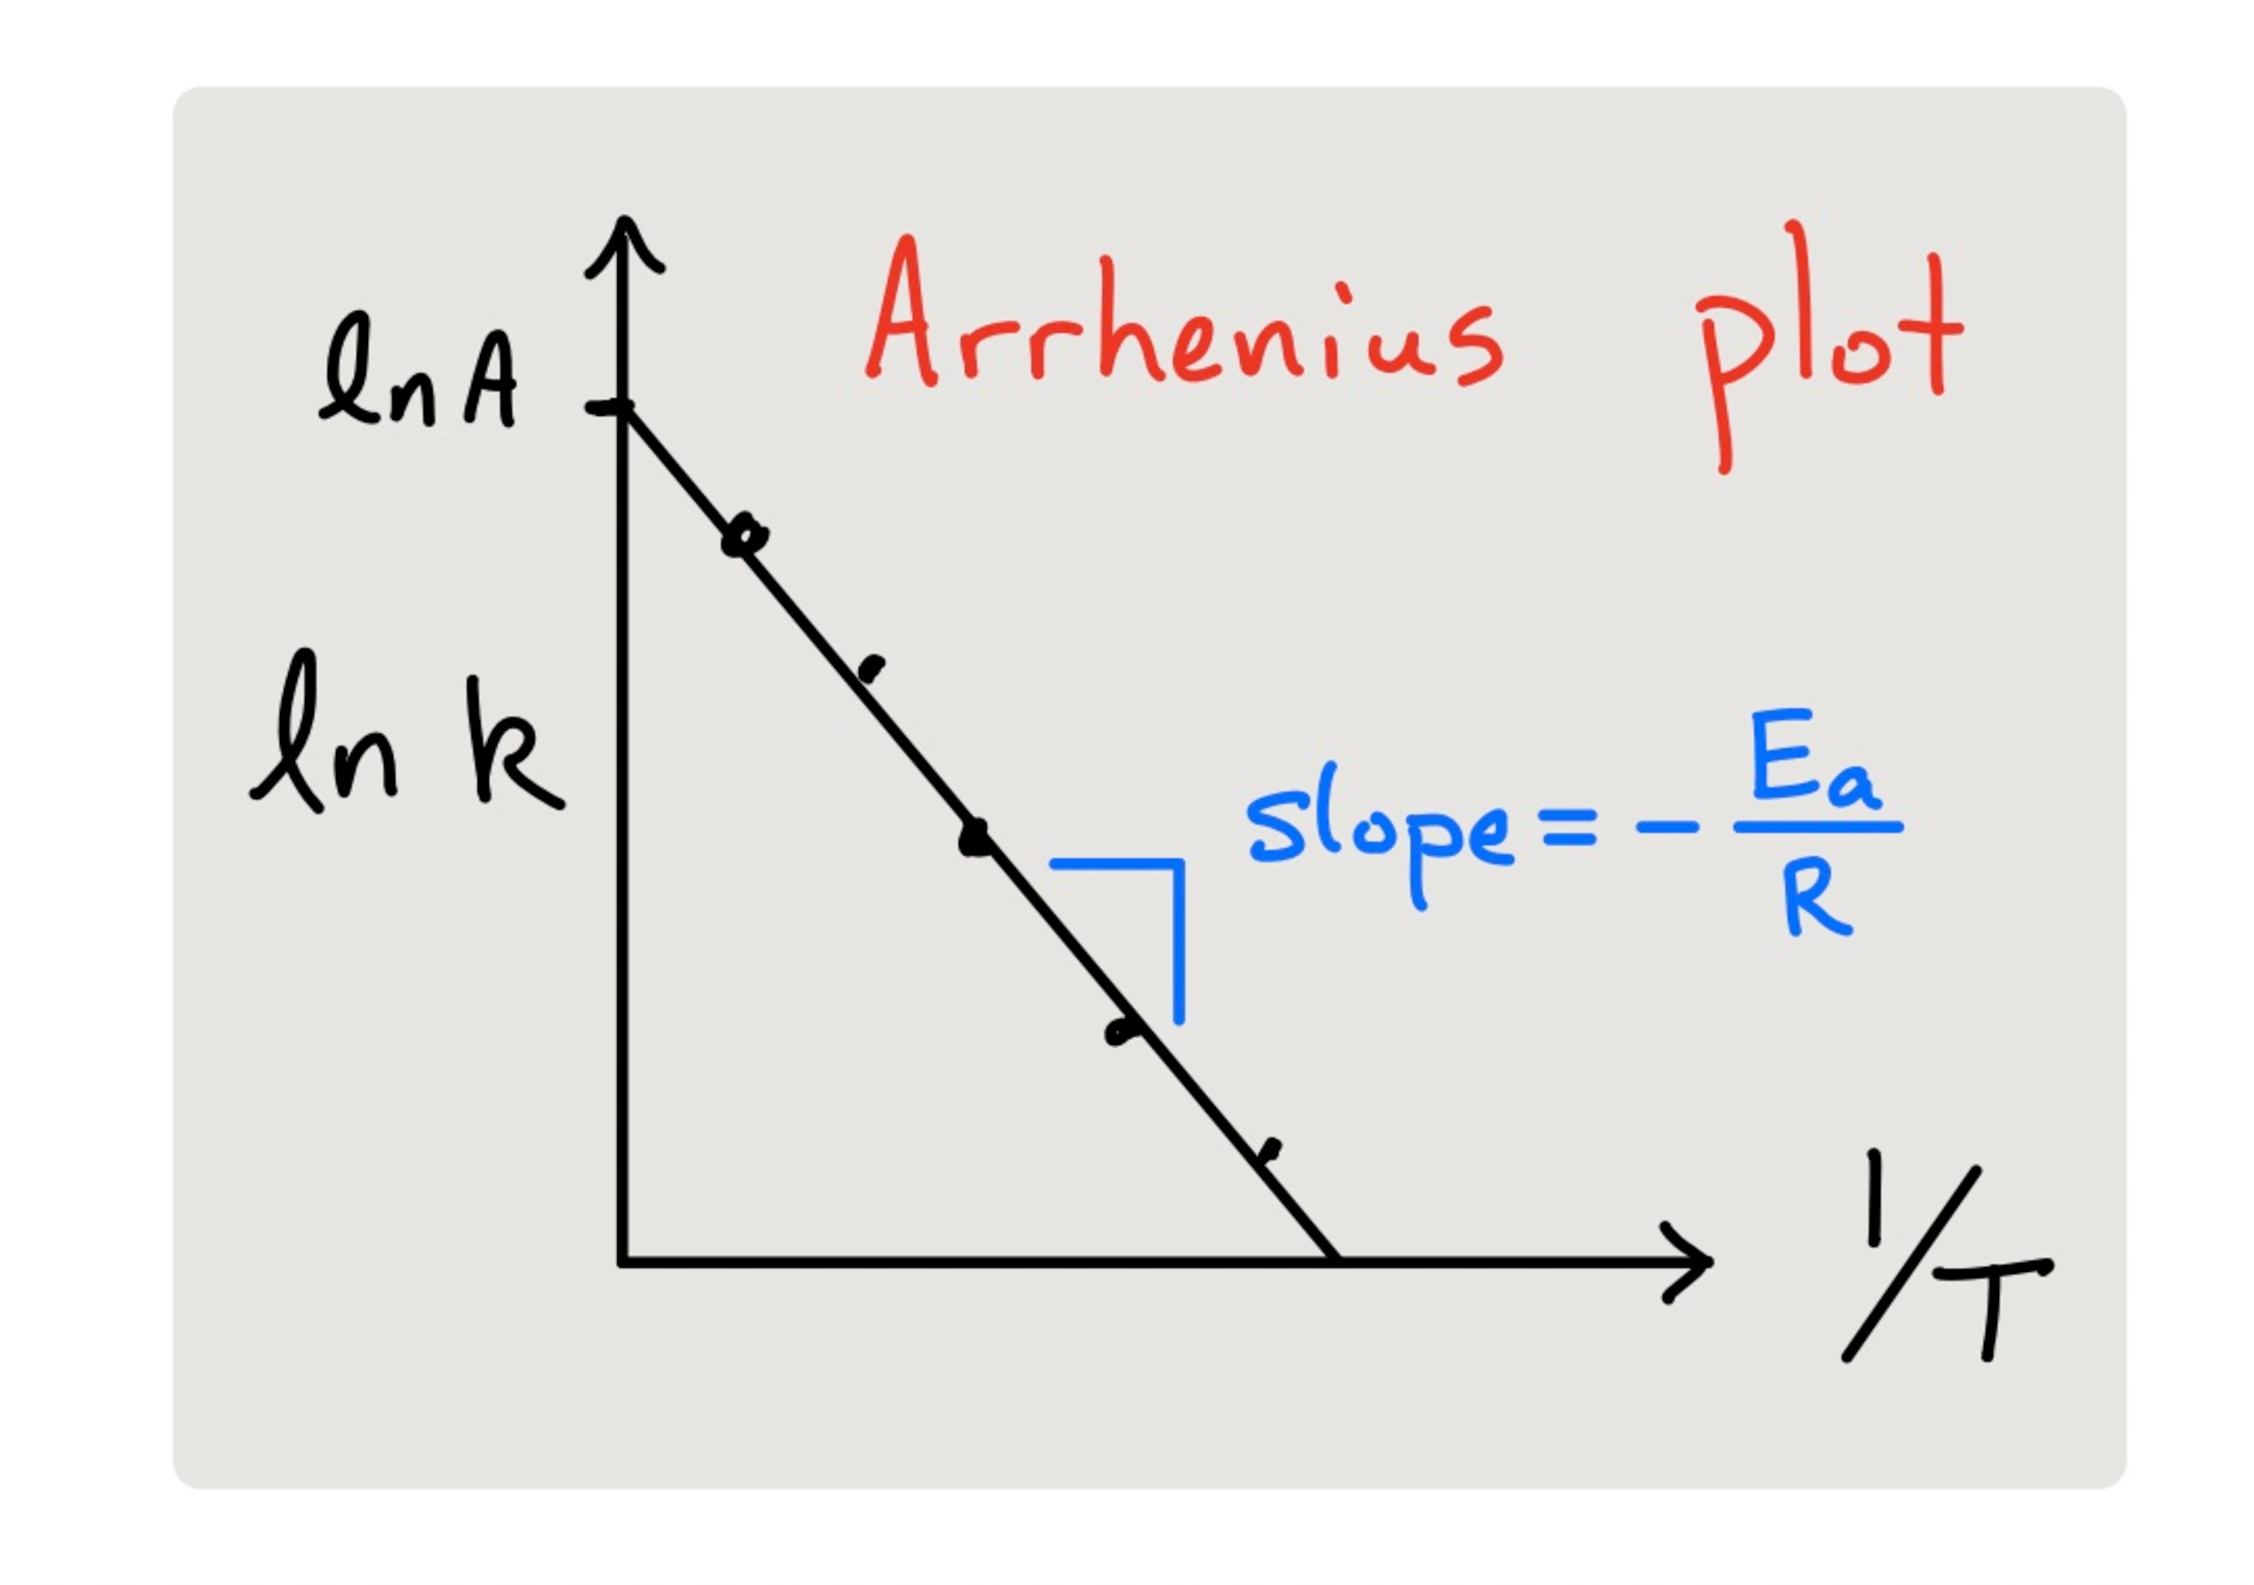
\includegraphics[width=0.8\linewidth]{src/7_Kinetics/images/arrhenius_plot.pdf}}
        \end{minipage}
    \end{minipage}
    
    \vspace*{0.5em}